\section{Usage example}

In this section, I will provide a full example of creating, designing, and publishing a website in the developed SaaS system from a user's perspective.

First, let me quickly go through the prerequisites.
I am going to assume the user already successfully obtained an account to the application.
Not only that, I expect that they already managed to verify their email, which is required for managing the website.

First, the user navigates to the sites page where at first, there is only an empty prompt signifying the user has not yet created a site.
Let's create a site, that for the example's sake, showcases the imaginary user's hobbies.
The site's name will be 'My hobby site'.

Figure \ref{fig:example-create} showcases these first two steps.
Subfigure \ref{subfig:example-empty} shows the empty page, while Subfigure \ref{subfig:example-new} displays the creation form.

\begin{figure}[H]
  \centering
  \begin{subfigure}[b]{0.49\textwidth}
    \centering
    \includegraphics[width=\textwidth]{./figures/example/example-1.png}
    \caption{Empty sites view}
    \label{subfig:example-empty}
  \end{subfigure}
  \hfill
  \begin{subfigure}[b]{0.49\textwidth}
    \centering
    \includegraphics[width=\textwidth]{./figures/site-pages.png}
    \caption{Example site creation}
    \label{subfig:example-new}
  \end{subfigure}
  \caption{Creating an example site}
  \label{fig:example-create}
\end{figure}

Next, the created page shows up in the sites list.
Let's edit its autogenerated homepage to be instead called 'Welcome'.
This is shown in Figure \ref{fig:example-update}, in which Subfigure \ref{subfig:example-list} shows the newly created site appearing in the list and Subfigure \ref{subfig:example-page-update} shows the page update form.

\begin{figure}[H]
  \centering
  \begin{subfigure}[b]{0.49\textwidth}
    \centering
    \includegraphics[width=\textwidth]{./figures/example/example-3.png}
    \caption{Example site in the list}
    \label{subfig:example-list}
  \end{subfigure}
  \hfill
  \begin{subfigure}[b]{0.49\textwidth}
    \centering
    \includegraphics[width=\textwidth]{./figures/example/example-4.png}
    \caption{Page update}
    \label{subfig:example-page-update}
  \end{subfigure}
  \caption{Updating a site's page}
  \label{fig:example-update}
\end{figure}

Continuing, let me create a new page for the hobby site.
Filling the multi-step form, let's name it 'Games' and give it the path \texttt{/games}.
Then, I chose to base it off of a schema and selected an example schema called 'Title with cards'.
At the final step, I reviewed my selection and saved the page.

This process, with each step outlined is in Figure \ref{fig:example-page-create-1} and Figure \ref{fig:example-page-create-2}.
Subfigure \ref{subfig:example-page-create-1} shows entering the detail of the new page, while Subfigure \ref{subfig:example-page-create-2} shows choosing between an empty or schema based page.
Subfigure \ref{subfig:example-page-create-3} displays the list of schemas a user can choose from and Subfigure \ref{subfig:example-empty} shows the review of the process.
\begin{figure}[H]
  \centering
  \begin{subfigure}[b]{0.49\textwidth}
    \centering
    \includegraphics[width=\textwidth]{./figures/example/example-5.png}
    \caption{Details}
    \label{subfig:example-page-create-1}
  \end{subfigure}
  \hfill
  \begin{subfigure}[b]{0.49\textwidth}
    \centering
    \includegraphics[width=\textwidth]{./figures/example/example-6.png}
    \caption{Schema as a base}
    \label{subfig:example-page-create-2}
  \end{subfigure}
  \caption{Creating a new page, first two steps}
  \label{fig:example-page-create-1}
\end{figure}

\begin{figure}[H]
  \centering
  \begin{subfigure}[b]{0.49\textwidth}
    \centering
    \includegraphics[width=\textwidth]{./figures/example/example-7.png}
    \caption{Selecting a schema}
    \label{subfig:example-page-create-3}
  \end{subfigure}
  \hfill
  \begin{subfigure}[b]{0.49\textwidth}
    \centering
    \includegraphics[width=\textwidth]{./figures/example/example-8.png}
    \caption{Reviewing}
    \label{subfig:example-page-create-4}
  \end{subfigure}
  \caption{Creating a new page, last two steps}
  \label{fig:example-page-create-2}
\end{figure}

Afterwards, the newly created page appears in the page list of the hobby website. Let's enter its details, which shows the preview of the page (the selected schema), details and controls.
Figure \ref{fig:example-page-list} shows these steps.
Subfigure \ref{subfig:example-page-list} shows the page in the site's page list, while Subfigure \ref{subfig:example-page-detail} presents the page's detailed view.

\begin{figure}[H]
  \centering
  \begin{subfigure}[b]{0.49\textwidth}
    \centering
    \includegraphics[width=\textwidth]{./figures/example/example-9.png}
    \caption{Page list}
    \label{subfig:example-page-list}
  \end{subfigure}
  \hfill
  \begin{subfigure}[b]{0.49\textwidth}
    \centering
    \includegraphics[width=\textwidth]{./figures/example/example-10.png}
    \caption{Page detail}
    \label{subfig:example-page-detail}
  \end{subfigure}
  \caption{Newly created page's detail and list view}
  \label{fig:example-page-list}
\end{figure}

Let me suggest some possible designs for both pages, which are displayed in Figure \ref{fig:example-design}.
Subfigure \ref{subfig:example-design-welcome} presents the design of the welcome page, containing cards for each interest of the user and some cat pictures at the bottom.
In contrast, Subfigure \ref{subfig:example-design-games} presents some of their favourite games in a similar fashion.

\begin{figure}[H]
  \centering
  \begin{subfigure}[b]{0.49\textwidth}
    \centering
    \includegraphics[width=\textwidth]{./figures/example/example-11.png}
    \caption{Welcome page}
    \label{subfig:example-design-welcome}
  \end{subfigure}
  \hfill
  \begin{subfigure}[b]{0.49\textwidth}
    \centering
    \includegraphics[width=\textwidth]{./figures/example/example-12.png}
    \caption{Games page}
    \label{subfig:example-design-games}
  \end{subfigure}
  \caption{Example designs}
  \label{fig:example-design}
\end{figure}

Then, let's return to the site's detail view and deploy the page with the provided controls.
Figure \ref{fig:example-deploy} presents the publish dialog asking for confirmation.

\begin{figure}[H]
  \centering
  \includegraphics[width=\linewidth]{./figures/example/example-13.png}
  \caption{Deploying the example page}
  \label{fig:example-deploy}
\end{figure}

Finally, in my local development environment the published site can be visited. Figure \ref{fig:example-published} shows the two pages accessible on \texttt{hobby.localhost}.
Subfigure \ref{subfig:example-published-welcome} shows the welcome page, and Subfigure \ref{subfig:example-published-games} presents the games page.

\begin{figure}[H]
  \centering
  \begin{subfigure}[b]{0.49\textwidth}
    \centering
    \includegraphics[width=\textwidth]{./figures/example/example-14.png}
    \caption{Welcome deployed}
    \label{subfig:example-published-welcome}
  \end{subfigure}
  \hfill
  \begin{subfigure}[b]{0.49\textwidth}
    \centering
    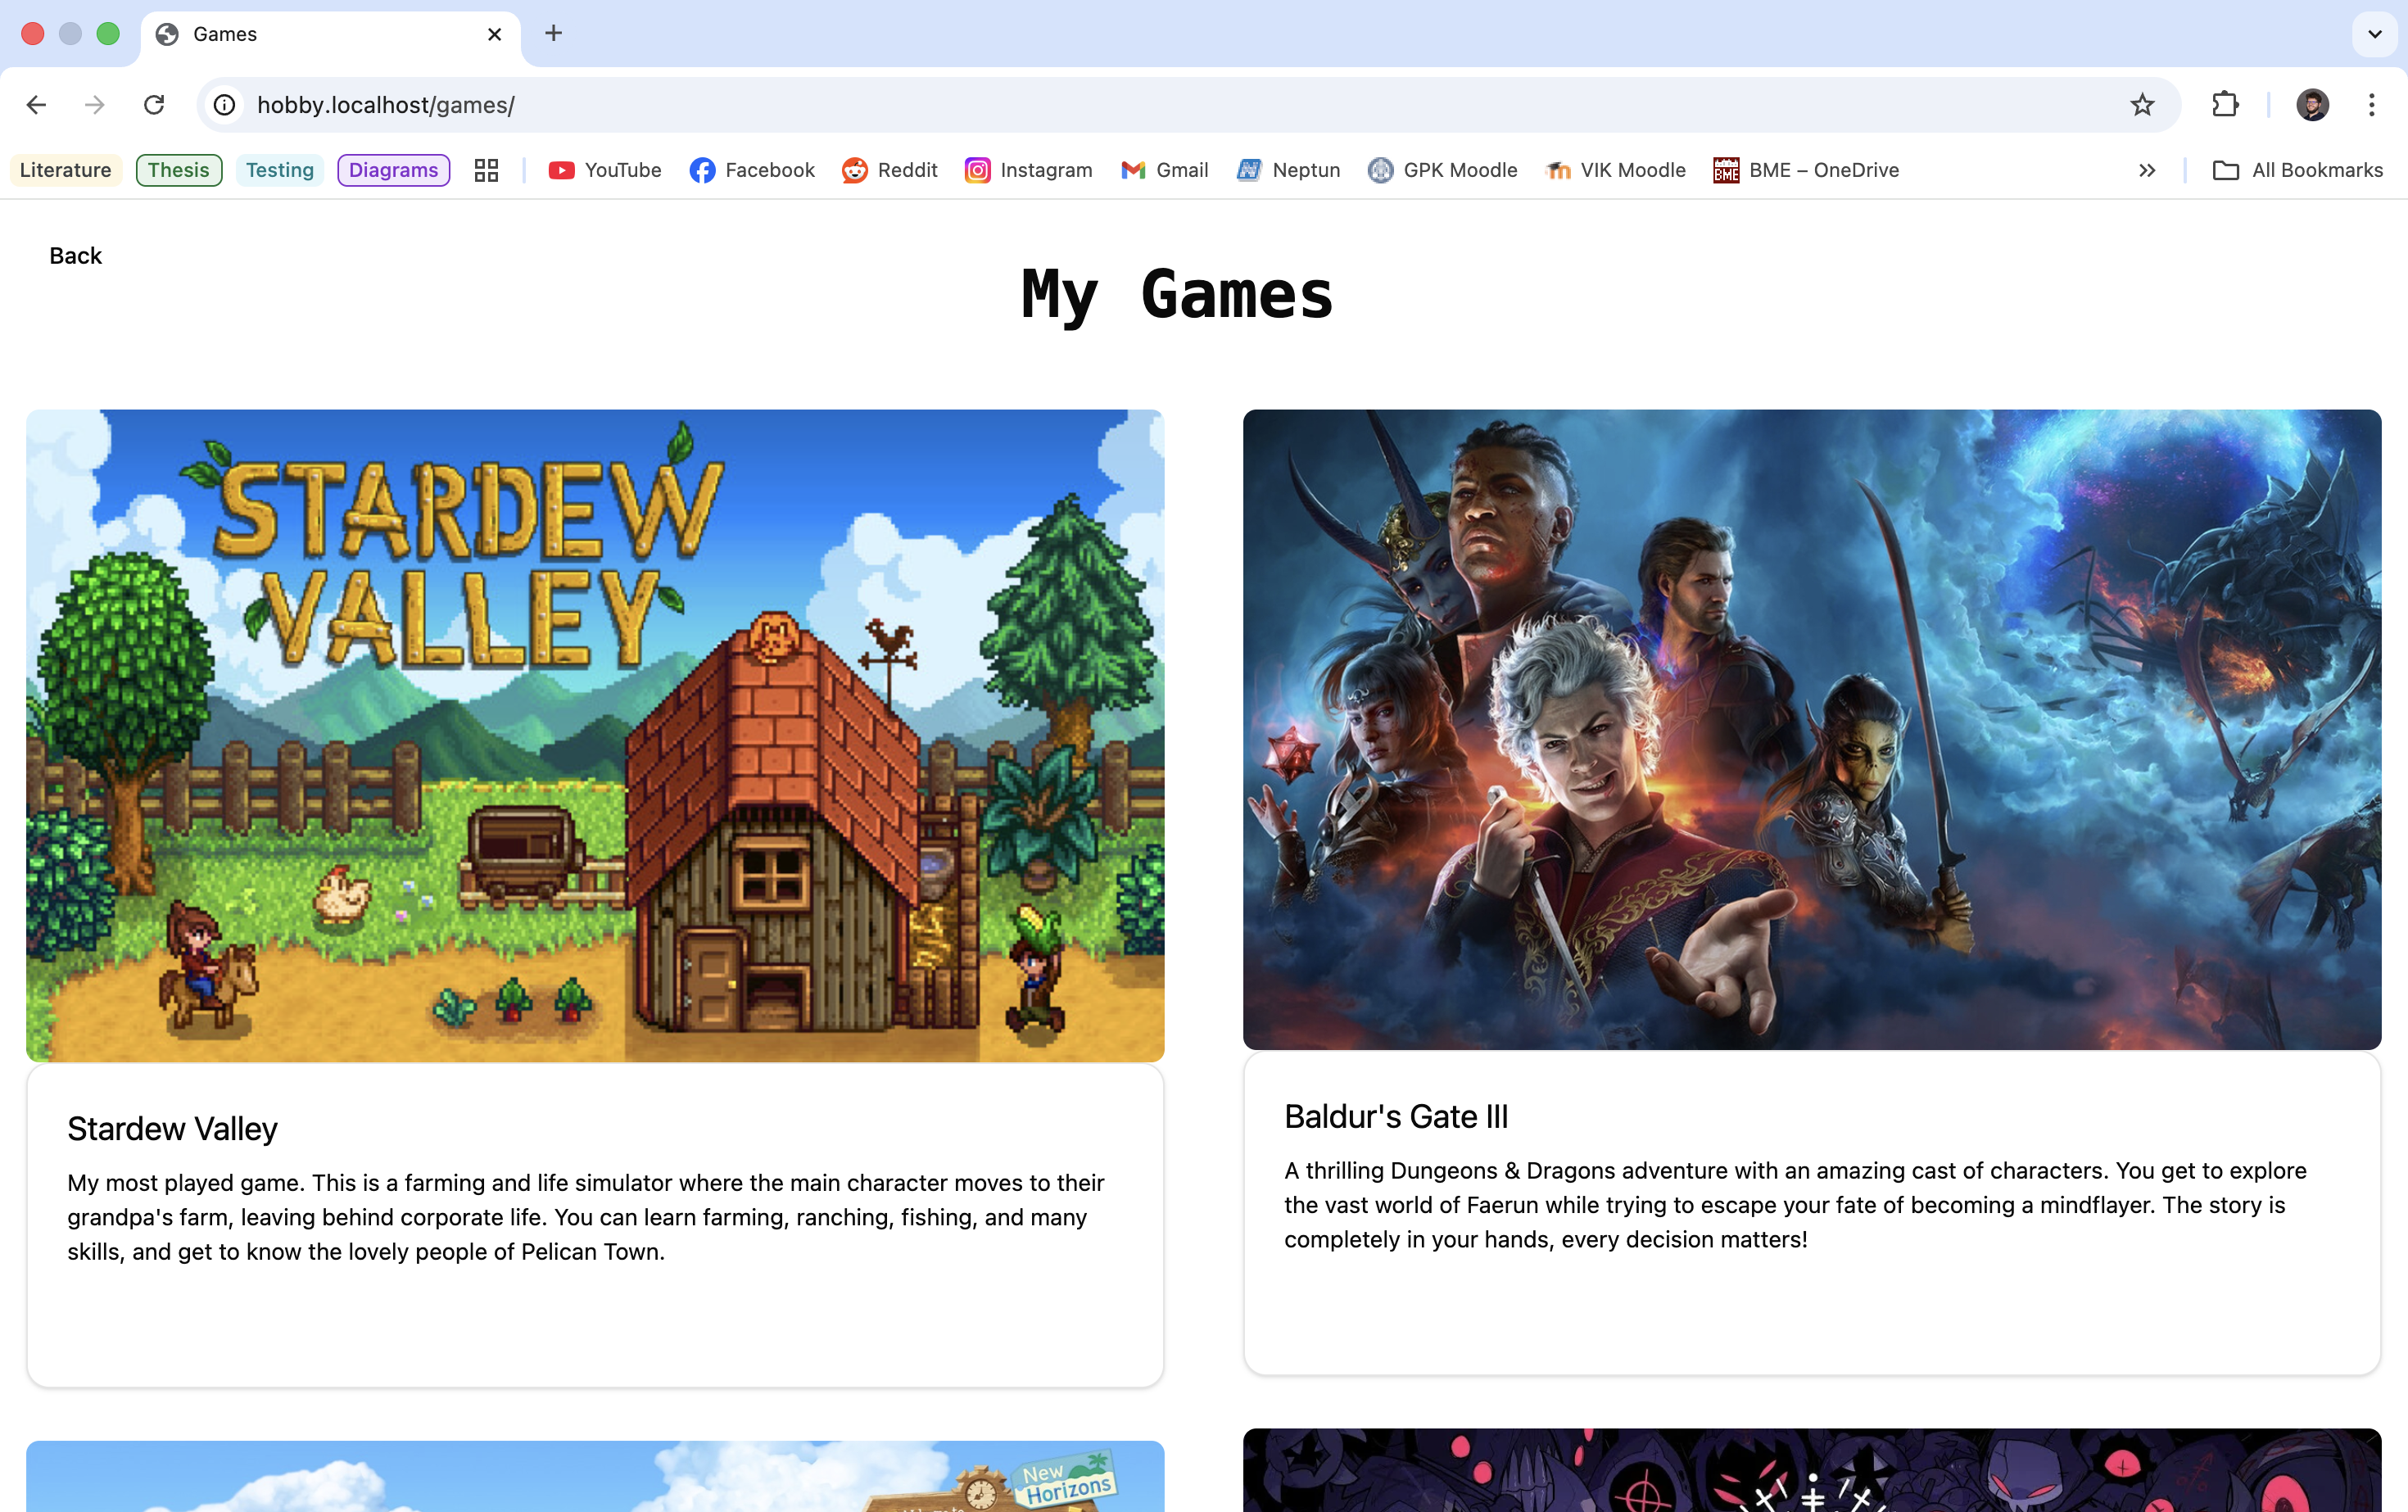
\includegraphics[width=\textwidth]{./figures/example/example-15.png}
    \caption{Games deployed}
    \label{subfig:example-published-games}
  \end{subfigure}
  \caption{Example site deployed}
  \label{fig:example-published}
\end{figure}

I will stop the example here, as it already showcases the main functionalities and capabilities of the application.
However, based on this short demo, it is easy to see how an end user may use the SaaS platform.
It can also be imagined that the user could easily follow these steps again, for example to edit this page further and redeploy the changes for others to see.